\XtoCBlock{Minimum}
\label{block:Minimum}
\begin{figure}[H]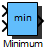
\includegraphics{Minimum}\end{figure} 

\begin{XtoCtabular}{Inports}
In1 & Input \#1\tabularnewline
\hline
In2 & Input \#2\tabularnewline
\hline
\end{XtoCtabular}


\begin{XtoCtabular}{Outports}
Out & Minimum of Input \#1 and Input \#2\tabularnewline
\hline
\end{XtoCtabular}

\subsubsection*{Description:}
Outputs the lesser value of the two input signals.

% include optional documentation file
\InputIfFileExists{\XcHomePath/Library/General/Doc/Minimum_Info.tex}{\vspace{1ex}}{}

\subsubsection*{Implementations:}
\begin{tabular}{l l}
\textbf{FiP8} & 8 Bit Fixed Point Implementation\tabularnewline
\textbf{FiP16} & 16 Bit Fixed Point Implementation\tabularnewline
\textbf{FiP32} & 32 Bit Fixed Point Implementation\tabularnewline
\textbf{Float32} & 32 Bit Floating Point Implementation\tabularnewline
\textbf{Float64} & 64 Bit Floating Point Implementation\tabularnewline
\end{tabular}

\XtoCImplementation{FiP8}
\index{Block ID!352}
\nopagebreak[0]
% Implementation details
\begin{tabular}{l l}
\textbf{Name} & FiP8 \tabularnewline
\textbf{ID} & 352 \tabularnewline
\textbf{Revision} & 0.1 \tabularnewline
\textbf{C filename} & Minimum\_FiP8.c \tabularnewline
\textbf{H filename} & Minimum\_FiP8.h \tabularnewline
\end{tabular}
\vspace{1ex}

8 Bit Fixed Point Implementation

% Implementation data structure
\XtoCDataStruct{Data Structure:}
\begin{lstlisting}
typedef struct {
     uint16        ID;
     int8          *In1;
     int8          *In2;
     int8          Out;
} MINIMUM_FIP8;
\end{lstlisting}

\ifdefined \AddTestReports
\InputIfFileExists{\XcHomePath/Library/General/Doc/Test_Minimum_FiP8.tex}{}{}
\fi
\XtoCImplementation{FiP16}
\index{Block ID!353}
\nopagebreak[0]
% Implementation details
\begin{tabular}{l l}
\textbf{Name} & FiP16 \tabularnewline
\textbf{ID} & 353 \tabularnewline
\textbf{Revision} & 0.1 \tabularnewline
\textbf{C filename} & Minimum\_FiP16.c \tabularnewline
\textbf{H filename} & Minimum\_FiP16.h \tabularnewline
\end{tabular}
\vspace{1ex}

16 Bit Fixed Point Implementation

% Implementation data structure
\XtoCDataStruct{Data Structure:}
\begin{lstlisting}
typedef struct {
     uint16        ID;
     int16         *In1;
     int16         *In2;
     int16         Out;
} MINIMUM_FIP16;
\end{lstlisting}

\ifdefined \AddTestReports
\InputIfFileExists{\XcHomePath/Library/General/Doc/Test_Minimum_FiP16.tex}{}{}
\fi
\XtoCImplementation{FiP32}
\index{Block ID!354}
\nopagebreak[0]
% Implementation details
\begin{tabular}{l l}
\textbf{Name} & FiP32 \tabularnewline
\textbf{ID} & 354 \tabularnewline
\textbf{Revision} & 0.1 \tabularnewline
\textbf{C filename} & Minimum\_FiP32.c \tabularnewline
\textbf{H filename} & Minimum\_FiP32.h \tabularnewline
\end{tabular}
\vspace{1ex}

32 Bit Fixed Point Implementation

% Implementation data structure
\XtoCDataStruct{Data Structure:}
\begin{lstlisting}
typedef struct {
     uint16        ID;
     int32         *In1;
     int32         *In2;
     int32         Out;
} MINIMUM_FIP32;
\end{lstlisting}

\ifdefined \AddTestReports
\InputIfFileExists{\XcHomePath/Library/General/Doc/Test_Minimum_FiP32.tex}{}{}
\fi
\XtoCImplementation{Float32}
\index{Block ID!355}
\nopagebreak[0]
% Implementation details
\begin{tabular}{l l}
\textbf{Name} & Float32 \tabularnewline
\textbf{ID} & 355 \tabularnewline
\textbf{Revision} & 0.1 \tabularnewline
\textbf{C filename} & Minimum\_Float32.c \tabularnewline
\textbf{H filename} & Minimum\_Float32.h \tabularnewline
\end{tabular}
\vspace{1ex}

32 Bit Floating Point Implementation

% Implementation data structure
\XtoCDataStruct{Data Structure:}
\begin{lstlisting}
typedef struct {
     uint16        ID;
     float32       *In1;
     float32       *In2;
     float32       Out;
} MINIMUM_FLOAT32;
\end{lstlisting}

\ifdefined \AddTestReports
\InputIfFileExists{\XcHomePath/Library/General/Doc/Test_Minimum_Float32.tex}{}{}
\fi
\XtoCImplementation{Float64}
\index{Block ID!356}
\nopagebreak[0]
% Implementation details
\begin{tabular}{l l}
\textbf{Name} & Float64 \tabularnewline
\textbf{ID} & 356 \tabularnewline
\textbf{Revision} & 0.1 \tabularnewline
\textbf{C filename} & Minimum\_Float64.c \tabularnewline
\textbf{H filename} & Minimum\_Float64.h \tabularnewline
\end{tabular}
\vspace{1ex}

64 Bit Floating Point Implementation

% Implementation data structure
\XtoCDataStruct{Data Structure:}
\begin{lstlisting}
typedef struct {
     uint16        ID;
     float64       *In1;
     float64       *In2;
     float64       Out;
} MINIMUM_FLOAT64;
\end{lstlisting}

\ifdefined \AddTestReports
\InputIfFileExists{\XcHomePath/Library/General/Doc/Test_Minimum_Float64.tex}{}{}
\fi
